\chapter{Application Prototype}
\label{ch:Prototype}
Before making a start on of the implementation phase, a lot of effort was put into the creation of the application prototype. Prototyping is a process of developing the initial model of the future application in order to determine the correct application structure, its functionality and the general concept. A prototype is just a model and may differ from the final product.

The project requirements outlined in the previous chapter of this report were used in order to create a mind map representing pages of the future application. This helped understanding what exactly is expected to be seen on each page of the website and what is the user journey in terms of the navigation. Wireframes were created for all the pages of the website. For this purpose was used just paper and pencils to aim flexibility.

In terms of the methodology, a hybrid of Agile and the traditional Waterfall approach was used for this project. Speaking of the traditional Waterfall approach, some of planning was made beforehands, for example requirements specifications, use-case diagrams, wireframes, etc. On the other hand, for the whole implementation phase was used test-driven approach that utilises the best of the agile techniques.

In general, Agile methodology focuses on team communication and project transparency. Nevertheless, one of its advantages is an extreme flexibility, therefore most of the basic components of Agile can still be effectively used by a single person. The key feature of the version of Agile adopted for the project was breaking down the project workload into clearly defined units of work (high-level features introduced in the chapter "Requirements Analysis" \ref{ch:requirementanalysis}), each associated with an iteration, and setting a milestone for each of them. Excel sheets were used for defining the set of tasks for each iteration. GitHub issue tracker was also used as a supporting productivity tool for this project. Code related tasks were recorded as "issues" for the project GitHub repository. The GitHub issue tracker appeared to be a very efficient tool for keeping the focus. TDD or test driven develoment was another key Agile technique adopted for the project. The unit tests covering business logic were always written before the implementation and the next sprint has not been started unless all tests from the previous sprint passed. 

In summary, in this section will be described the process of transforming project requirements into the system design. Several design cornerstones (website structure mind map, a set of wireframes) were produced beforehands. Other elements of the application design (use cases, database schema) were updated in iterations, inline with the Agile methodology. 

\section{Application Structure}
\label{sec:applicationstructure_prototype}
The prototyping process started with producing a large mind map of the future application.  I found mindmapping a very useful way to brainstorm on my ideas, capture and organise them. The final version of the diagram puts together the structure of application pages, navigation scenarios and other ideas relevant to the design. A full mind map can be found in the figure below.

\begin{figure}[H]
	\begin{center}
		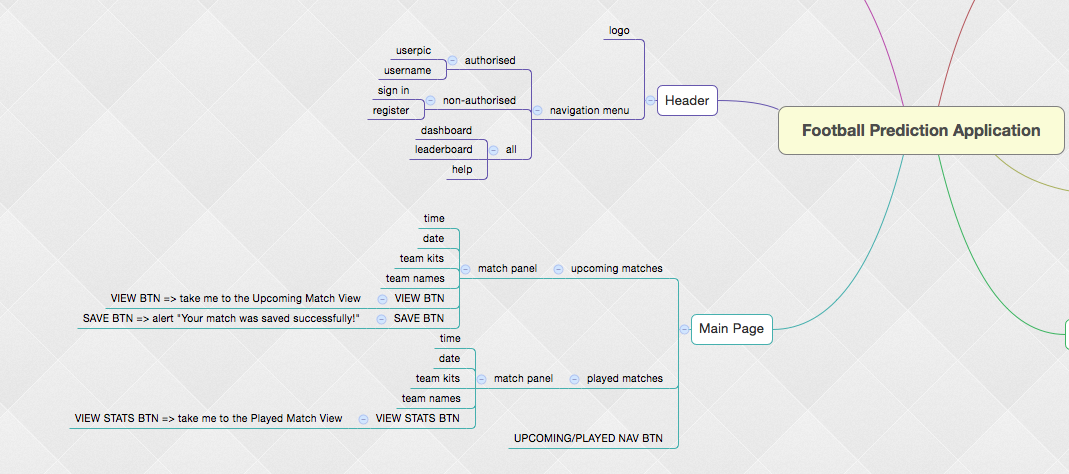
\includegraphics[width=.90\textwidth]{design/images/mindmap}
		\caption{Mind map capturing the result of the initial brainstorming on the application structure and navigation scenarios.} \label{fig:using:mindmap}
	\end{center}
\end{figure}

\section{Inspiration}
\label{sec:inspiration_prototype}
As the next step, I took another look at the currently available websites, hoping to get some ideas on how to approach the visual side of the project and to improve its usability. This step is an important stage of an application prototyping process: it allows to learn from the best design practices and possibly avoid potential errors. The usual practice is to first concentrate on several websites of the direct competition. However, the future application does not really have any direct competitors, as the idea behind the project is quite new. Therefore, I concentrated on the football statistics and news websites (listed in the chapter \ref{ch:Requirements Analysis}, subsection "Current Solutions") making a note of how those websites present football statistics to their users.

\section{Wireframes}
\label{sec:wireframes_prototype}
When speaking about prototyping, in the early stages the first choice of many designers is often a piece of paper and a pencil. Sketching has a number of advantages when compared to the use of the editors, such as Fireworks or Photoshop. When using editors, it is easy to get distracted by brushing up unnecessary details too early. On the opposite side, sketches offer a lot of flexibility. It is easy to add notes, make small changes or replace an outdated sketch with a fresh one.

In case of this project, each of the sketches represented a separate “view” of the website. The scale of a “view” might differ. For example, some sketches show a whole page (home page, dashboard page, etc.), others just showed certain blocks of the website, such as header, footer, user profile container in more detail. I always added a lot of comments to explain the navigation and sometimes expected output. Sketches were one of the most powerful tools I used during the prototyping process. 


Scans of the drawings

\section{Visual Design: Branding, icons, Font}
\label{sec:visdesign_prototype}
First website prototype in a photoshop/Fireworks
Early prototype using html and css, using bootstrap should be quick and easy

The project clearly needs an identity. As a placeholder, I created a logo a couple of weeks ago, entitled “SureThing”. It seemed a fairly good and appropriate name: my platform offers ..., but in a smart way, ... user driven prediction..


Branding - number of names for the application
Bootstrap was used as a framework on the front-end.
Flat design is a big trend of the last years. It was decided to use the flat design in order to not distract user from the content.
The design is a mixture of free templates and UI freebies created specifically for Bootstrap.

\section{Use Cases}
\label{usecases_prototype}
As mentioned above, use cases and the database diagram presented below, were prototyped in iterations. In this report will be presented a completed, merged version of the set of use cases and the database design. For use cases UML will be used to design in a clear and readable manner.

\section{Database Design}
\label{databasedesign}
what database was used
Use this link to describe the ORM and its advantages: 
http://www.aosabook.org/en/sqlalchemy.html

\subsection{Database Schema}
Describe how the database was designed (what we need to capture and how I gradually added table by table). Start with user, as it is the cornerstone of the application (see forthergill)
The database class diagram presented is a result of numerous iterations.  
Present also database before and after.

\subsection{Database Class Diagram}

